%!TEX root = ../thesis.tex



\chapter{Practical performance}
\label{chap:pracPerf}
\section{Setup}
\label{sec:Setup}
In this chapter we will examine the practical relative performance of the three algorithms. We will do so in several ways. The first way is with the use of simulated data (recreated from \cite{Hastie2009}). We have ten features $X_1,\ldots,X_{10}$ which are drawn from a standard independent Gaussian. Their label is determined (deterministically) by the following rule: $$Y:=\begin{cases}
1 & \text{ if } \sum_{k=1}^{10} (X_k)^2 > \chi_{10}^2(0.5)\\
-1 & \text{otherwise}
\end{cases}$$ Where $\chi_{10}^2(0.5)=9.34$ is the median of a chi-squared random variable with ten degrees of freedom. This is to ensure that there are roughly the same amount of labels in each category. 

\par The second way we will test the algorithms is the UCI ``a9a Adult dataset'' \cite{LIBSVM}. Here the goal is to predict whether an individual will earn more than \$50,000 per year or not. The original data set has 14 features, among which six are continuous and eight are categorical. In this data set, continuous features are discretized into quantiles, and each quantile is represented by a binary feature. Furthermore a categorical feature with $m$ categories is converted to $m$ binary features. 

\par In an attempt to keep the comparison as consistent as possible we will, in all settings, use 32,561 observations for training and 16,281 for testing. This is because these are the amount of observations in the a9a data set. This ratio of training to testing observations is not uncommon. Recall to avoid over fitting we cannot test the algorithm on the same dataset we use to train it, thus any observations which are used to test cannot be used to train, therefore this kind of ratio is desirable.

\par We implemented the algorithms in Python 3. Here we used Scikit-learn's implementation of a decision tree as our weak learner \cite{Pedregosa2012}. For the interested reader our implementations of all the algorithms discussed in this thesis, as well as everything necessary to recreate the experiments, is freely available at \url{https://github.com/dvente/bscthesis} 

\section{Datasets}
\subsection{\adaB}
\label{subsec:AdaPracPerf}
\begin{figure}[!ht]
  \centering
      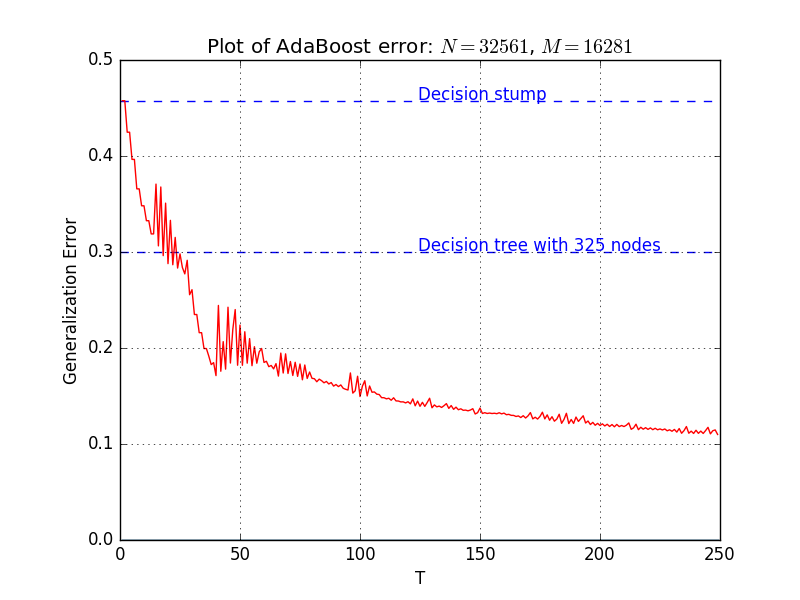
\includegraphics[width=\graphWidth]{generated/ADGD.png}
  \caption{Generalization error of AdaBoost as a function of the number of iterations over the simulated data set. The error rate of the decision stump and a decision tree with 325 nodes are shown for reference}
      \label{fig:adaBGD}
\end{figure}


\par Looking at figure \ref{fig:adaBGD} it is obvious that \adaB works. The decision stump initially performs with an error rate of 47\% which is indeed only slightly better than random guessing. \adaB outperforms this and even a large tree with 325 nodes and an error rate of 30\% after just tens of iterations and reaches an error rate as low as 7.7\% after 500 iterations.

\newpage
\par Considering figure \ref{fig:adaBSVM} below the situation is a bit different for the a9a data. One sees that the algorithm still works but here we run into some limitations. As we can see the initial stump performs significantly better to start with, with an error rate of 23.6\%. After just 50 iterations we see diminishing returns set in quite drastically, seeing only a slight improvement from 15.7\% to 15.2\% over the course of 450 iterations. Of course this also happens with the simulated data but to a much lesser degree. This is probably due to the fact that the simulated data is much more homogeneous, where in fact all features are equally important, with the hard examples being those where all features are small but just meet the criteria. The observed data however most likely has a few features that improve the accuracy a lot (for example education), but beyond that the data doesn't show any important examples so the gains, after to low hanging fruit have been picked, are marginal. While this is still a good result it is useful to keep this phenomenon in mind while we examine the rest of the algorithms. This characteristic highlights a fundamental disadvantage of a weak learner, namely that depending on the data set there might simply not be a way to improve the accuracy beyond a certain point. 

\par A final observation on the reference trees should be useful here: while we did try to keep the size of the trees as consistent as possible, it is quite hard to enforce a specific size over different data sets, especially ones that differ as strongly as our two data sets. This is why the  trees have slightly different sizes across the different plots. We attempted to keep the sizes as similar as possible by enforcing a maximum depth of $\lfloor \log_2(500)\rfloor=8$, letting the algorithms fit the trees as best possible under this constraint. We have chosen this because this ensures an upper bound of 500 nodes, which we found to be a reasonable bound for the size and shapes of our considered data.
\begin{figure}[!ht]
  \centering
      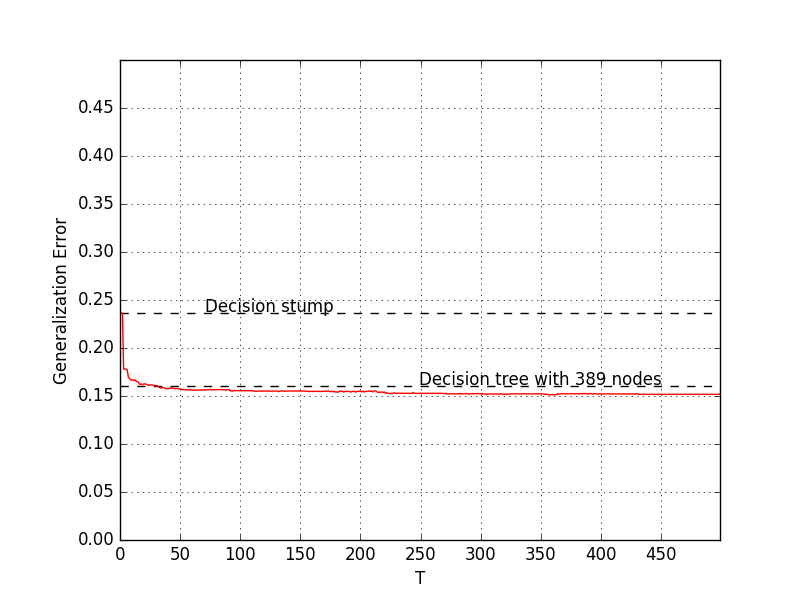
\includegraphics[width=\graphWidth]{generated/ADSVM.png}
  \caption{Generalization error of AdaBoost as a function of the number of iterations over the a9a data set. The error rate of the decision stump and a relatively large decision tree are again shown for reference}
      \label{fig:adaBSVM}
\end{figure}
\FloatBarrier

 \subsection{\NHB}
 \label{subsec:NHPracPerf}
Before we discuss the results of \NHB here we would like to highlight two important differences between \NHB and \adaB. The first is that to improve performance \NHB attempts to assign zero weight to unimportant examples in order to improve performance. The percentage of examples which were assigned weight zero is shown in green in the plots below. The second important difference is that whereas \adaB decides the label based on a reference threshold, \NHB simply takes an unweighted majority vote. A consequence of this is that on the even iterations the final committee might be tied on a decision. In an attempt to reflect this in our comparison we count the inconclusive tests (shown in a percentage of the testing size in blue) and recorded these as ``half a mistake'' since the committee was neither right nor wrong. Of course this impacts the performance of the algorithm quite significantly as can be seen below.  One important remark is that the committees are never tied in the case of an odd size. For the sake of clarity the graphs of the inconclusive tests in the plots below only show the percentage on the even iterations, those on the odd iterations always being 0.


\begin{figure}[!ht]
  \centering
      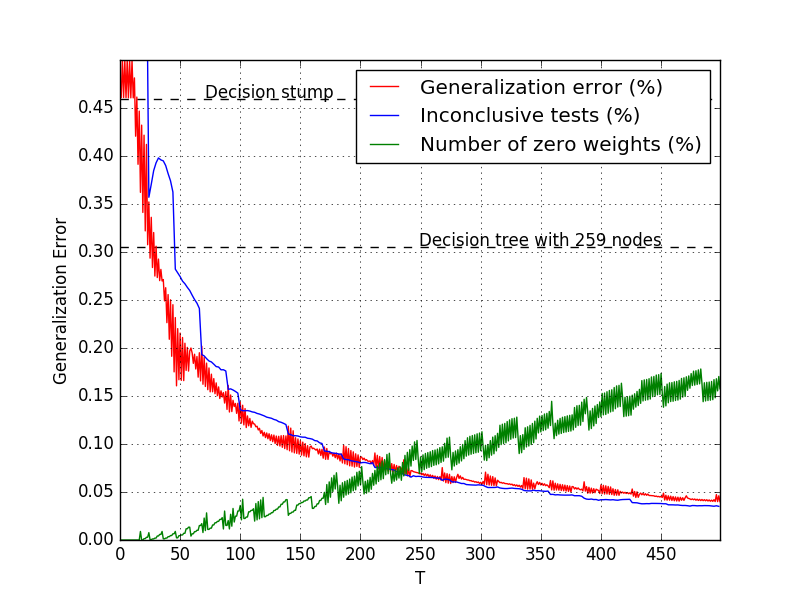
\includegraphics[width=\graphWidth]{generated/NHGD.png}
  \caption{Generalization error of \NHB as a function of the number of iterations on the simulated data. The error rates of trees with 3 and 259 nodes respectively are again shown for reference. It is important to remark that for clarities' sake we omitted the inconclusive data points of all odd iterations as they are always 0.}
      \label{fig:NHBGD}
\end{figure}
 \FloatBarrier
 \par The first thing one notices when looking at the above figure is that this mimics the behavior predicted by the theory, as well as the behavior of \adaB. The error rate as well as the percentage of inconclusive tests steadily decline while the percentage of zero weights steadily increase. In terms of actual percentages the algorithms perform quite similarly as was already studied in \cite{Luo2014}. Where \adaB achieved a error rate of 7.7\% after 500 iterations \NHB achieves 3.9\% which is much better. This is achieved by zero weight percentage of 15.7\% at the end. Since \NHB is the only algorithm that does this it isn't very useful for comparison's sake, but it is nice to see since it is quite a significant part which, again as we will see, improves performance quite a bit.  
\begin{figure}[!ht]
  \centering
      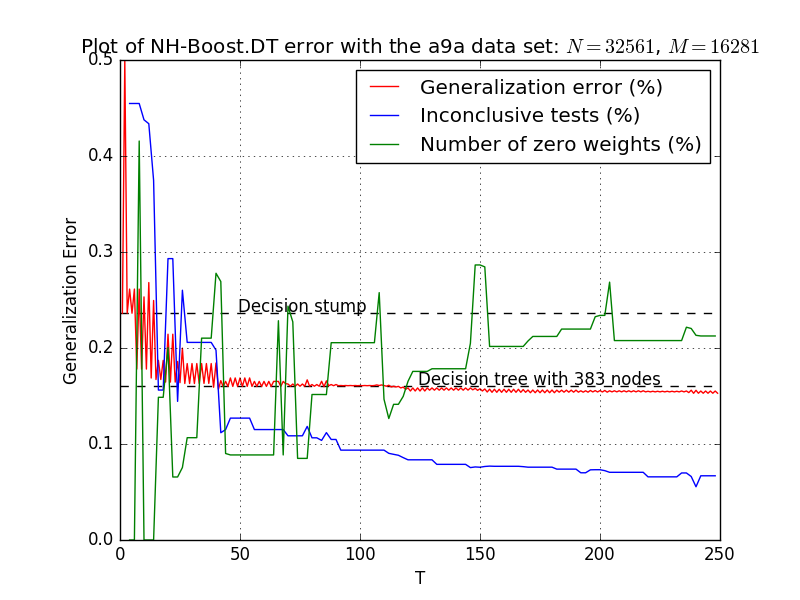
\includegraphics[width=\graphWidth]{generated/NHSVM.png}
  \caption{Generalization error of \NHB as a function of the number of iterations on the a9a data. The error rates of trees with 3 and 383 nodes resp. are again shown for reference. It is important to remark that for clarities' sake we omitted the inconclusive data points of all odd iterations as they are always 0.}
      \label{fig:NHBSVM}
\end{figure}

\par When looking at the observed data the story is again a bit different. The first obvious thing to note when looking at figure \ref{fig:NHBGD} is that the algorithm is (initially) quite confused about the amount of examples to assign a zero weight. One possible cause is that the weights of the previous round are determined by the performance of the previous iteration and that the algorithm gets slightly confused by the inconclusive tests. The peaks of zero weights are almost all around the 28\% whereas the last iteration has a zero weight percentage of 16.5\%. This compares quite favorably to the previous data set, which can be explained by our interpretation that after the low hanging fruit has been picked many examples become irrelevant and thus get assigned zero weight. One can, however, also wonder how reliable this interpretation is due to all the peaks and valleys. 
\par Here again we see the ``low hanging fruit'' characteristics we saw in the \adaB implementation. Here the final error rate bottoms out at 15.3\% compared to \adaB 15.4\% which is almost identical. One can wonder about the role the inconclusive tests play in this conclusion. This is however not of a big concern, since the accuracy on the odd iterations is also almost identical. Furthermore the inconclusive tests are an indication that the committee is not very certain on those predictions even if they aren't tied in the odd iterations. This tells us that these percentages are indeed very comparable.  
\FloatBarrier
\subsection{\squintB}
\label{subsec:sqPracPerf}
Finally we will consider \squintB. Looking at figure \ref{fig:SQGD} below we again see the predicted behavior. After some initial spikes both the error rate and the fraction of inconclusive tests steadily decline. As one can see it indeed performs incredibly similar to the other algorithms, finally achieving an error rate of 9.2\% compared to the 7.7\% and 3.9\% of \adaB and \NHB respectively. While it is still a good result, we must conclude that \squintB doesn't outperform \NHB or even \adaB in this setting. 
\begin{figure}[!ht]
  \centering
     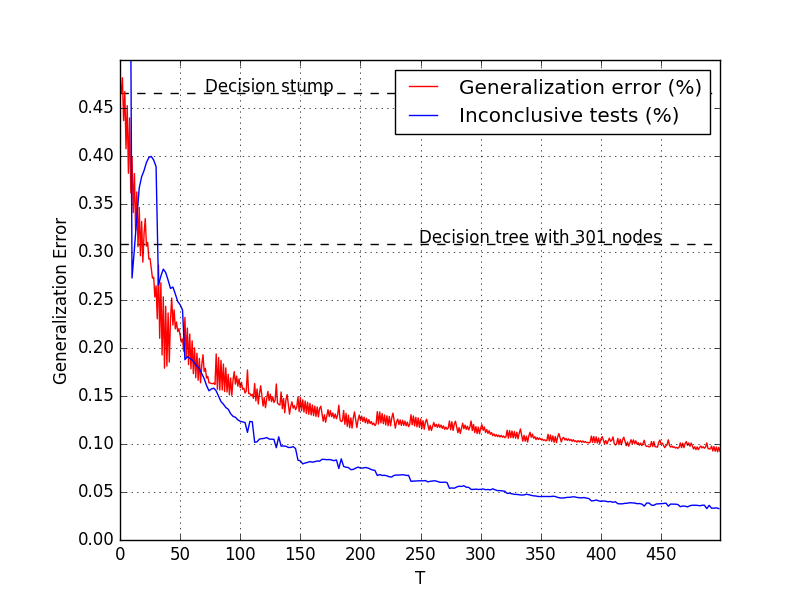
\includegraphics[width=\graphWidth]{generated/SQGD.png}
  \caption{Generalization error of \squintB as a function of the number of iterations on the simulated data. The error rates of trees with 3 and 301 nodes resp. are again shown for reference. It is important to remark that for clarities' sake we omitted the inconclusive data points of all odd iterations as they are always 0.}
      \label{fig:SQGD}
\end{figure}

\par When looking at figure \ref{fig:SQSVM} below of \squintB on the observed data, we again see the same behavior as with the other two algorithms. The initial improvement is quite fast but it bottoms out fairly quickly finally achieving an error rate of 15.04\% which is again extremely similar to the 15.4\% and 15.3\% of the other two algorithms. 


\begin{figure}[!ht]
  \centering
    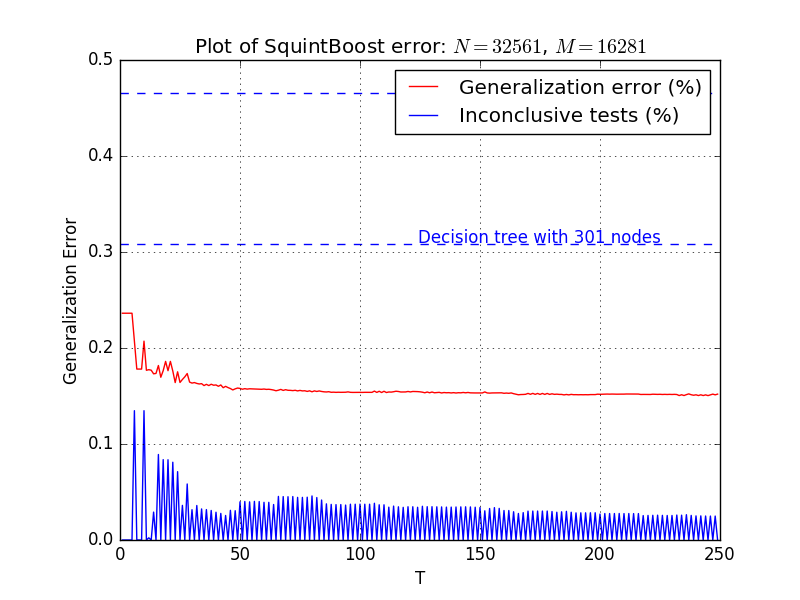
\includegraphics[width=\graphWidth]{generated/SQSVM.png}
  \caption{Generalization error of \squintB as a function of the number of iterations on the a9a data. The error rates of trees with 3 and 385 nodes resp. are again shown for reference. It is important to remark that for clarities' sake we omitted the inconclusive data points of all odd iterations as they are always 0.}
      \label{fig:SQSVM}
\end{figure}
\FloatBarrier


% \section{Computation}
% \label{sec:timed}

% Here we will finally describe the performance of the algorithms as a function of the computation time. Each of the algorithms was given a fixed amount of CPU time during which it was allowed to train. When the time elapsed the algorithm was allowed to finish its current iteration and was then tested on the same test data as before. This metric reflects real world performance slightly better than the iteration-wise comparison. This is true since if an algorithm performs worse per iteration but is faster then we can just run it for more iterations and get a better accuracy. We tested all the algorithms on both the data sets, the results of which can be found in table \ref{tbl:GDTime} and \ref{tbl:SVMTime} respectively.
% \begin{table}[htbp]
% \centering
% \begin{tabular}{|c|c|c|c|c|}
% \hline
% Algorithm & Execution time (s) & Iterations & Error (\%) & Inconclusive tests (\%)  \\ \hhline{|=|=|=|=|=|}
% \multirow{ 2}{*}{\adaB} & 1.194 & 5 & 39.64 & 0.00  \\\cline{2-5}
% & 60.122 & 241 &  11.11 & 0.00  \\ \Xhline{1pt}
% \multirow{ 2}{*}{\adaN} & 1.004 & 220 & 11.48  & 0.0 \\\cline{2-5}
% & 60.000 & 15407 &  6.99 & 0.18  \\ \Xhline{1pt}
% \multirow{ 2}{*}{\squintB} & 1.002 & 31 & 26.80  & 39.09\\\cline{2-5}
%  & 60.022 & 1711 &  7.56  &  1.02\\ \hline
% \end{tabular}
% \caption{Timed tests of the algorithms on the simulated data}
% \label{tbl:GDTime}
% \end{table}

% \begin{table}[htbp]
% \centering
% \begin{tabular}{|c|c|c|c|c|}
% \hline
% Algorithm & Execution time (s) & Iterations & Error (\%) & Inconclusive tests (\%)  \\ \hhline{|=|=|=|=|=|}
% \multirow{ 2}{*}{\adaB} & 1.167 & 6 & 17.68 & 0.00  \\\cline{2-5}
% & 60.192 & 297 &  15.25 & 0.00  \\ \Xhline{1pt}
% \multirow{ 2}{*}{\NHB} & 1.085 & 12 & 17.80  & 0.0 \\\cline{2-5}
% & 60.0120 & 578 &  15.14 & 0.0  \\ \Xhline{1pt}
% \multirow{ 2}{*}{\squintB} & 1.024 & 15 & 17.93  & 9.23\\\cline{2-5}
%  & 60.009 & 815 &  15.23  &  13.81\\ \hline
% \end{tabular}
% \caption{Timed tests of the algorithms on the a9a data}
% \label{tbl:SVMTime}
% \end{table}

% \par There are several observations to make here. In the tests over the simulated data \NHB significantly outperforms the other two algorithms in iterations in at least an order of magnitude and significantly better error rates in both time categories. \squintB is however still better than \adaB beating it again by almost an order of magnitude in both time categories and improving the error rate in both categories by 4\% in the 60s category and 12\% in the 1s category. It should be noted that 4\% in the former category is still quite significant because of the law of diminishing return. 
% \par When we consider the a9a data set the landscape looks somewhat different. While \squintB performs more iterations than the other two algorithms is has the highest error rate in both categories. We have already discusses the properties of this dataset so we won't go into detail about it again, but the main observation is that these differences aren't significant so we can largely dismiss these results. 

% \par Table \ref{tbl:SVMTime} does illustrate two other interesting things though. The first is that the iterations are much lower than with the simulated data. This is most likely due to the fact that the simulated data has only 10 features where as the observed data has 123 increasing the processing time quite a bit. In this scenario \squintB did perform significantly more iterations than the other two, suggesting that \squintB might outperform the other two algorithms if the data contains a lot of features but doesn't have the ``low hanging fruit'' problem that the a9a has. 

% \par Another important observation we can make is about the disadvantage of more iterations. As can be seen in tables \ref{tbl:GDTestingTime} and \ref{tbl:SVMTestingTime} respectively the time that it takes to test the algorithm on the same data set increases linearly with the computation time. This isn't a problem in and of itself but should be taken into consideration. Both the amount of features and the amount of iterations play a role in the computation time, as was to be expected. This means that when considering the algorithms one should not only take into account the number of features and how conducive the data is to boosting (does it have the low hanging fruit property?), but also how much time is a factor in the prediction phase. Namely if the predictions must be very quick then it might be better to take the algorithm that is slower but has to perform less iterations.  

% \begin{table}[htbp]
% \centering
% \begin{tabular}{|c|c|c|}
% \hline
% Algorithm & Execution time (s) & Testing time (s)  \\ \hhline{|=|=|=|}
% \multirow{ 2}{*}{\adaB} & 1.167 & 8.860 \\\cline{2-3}
% & 60.192 & 414.593  \\ \Xhline{1pt}
% \multirow{ 2}{*}{\NHB} & 1.085 & 92.030 \\\cline{2-3}
% & 60.0120 & 6453.419  \\ \Xhline{1pt}
% \multirow{ 2}{*}{\squintB} & 1.024 & 26.194\\\cline{2-3}
%  & 60.009 & 1474.809\\ \hline
% \end{tabular}
% \caption{Testing time of the algorithms on the simulated data}
% \label{tbl:GDTestingTime}
% \end{table}

% \begin{table}[htbp]
% \centering
% \begin{tabular}{|c|c|c|}
% \hline
% Algorithm & Execution time (s) & Testing time (s)  \\ \hhline{|=|=|=|}
% \multirow{ 2}{*}{\adaB} & 1.167 & 24.160 \\\cline{2-3}
% & 60.192 & 1038.695  \\ \Xhline{1pt}
% \multirow{ 2}{*}{\NHB} & 1.085 & 38.211 \\\cline{2-3}
% & 60.0120 & 1829.719  \\ \Xhline{1pt}
% \multirow{ 2}{*}{\squintB} & 1.024 & 47.742\\\cline{2-3}
%  & 60.009 & 1870.409\\ \hline
% \end{tabular}
% \caption{Testing time of the algorithms on the a9a data}
% \label{tbl:SVMTestingTime}
% \end{table}
% \FloatBarrier
 
\chapter{Conclusion and Future Work} 
\label{sec:Concl}

In this thesis we compared the practical performance of the three algorithms \adaB, \NHB and \squintB. We are not able to say that \squintB out performs the previous two algorithms. We used both a simulated dataset and a well known observed dataset to compare the algorithms. In the setting of an equal number of iterations \NHB came out the best with both the lowest error rate and the least inconclusive tests (where applicable). We also illustrated a possible problem with boosting. Namely that it might be possible that the data has a few obvious criteria which work fairly well but is very difficult to improve beyond those initial criteria, a property we called the low hanging fruit property, boosting might not be able to improve beyond a certain point while still increasing computation time in both the training and the predicting phase. 

\par Because of time constraints we were only able to compare the algorithms on two data sets. Future work could include the testing over a broader range of data, with both small and large shapes, that may or may not have the low haning fruit property. Furthermore it could try to devise certain tests to determine whether the data to be used is conducive to boosting. One of the problems \squintB and \NHB encounter is the problem of tied committees, so further work could include a search to break the ties in a meaningful way to potentially improve the accuracy of the algorithms, and to see if this indeed works. 
